\documentclass{bioinfo}
\usepackage{epstopdf}
\usepackage{url,color}
\copyrightyear{2015}
\pubyear{2015}

\usepackage{subfigure,bm,algorithm,algorithmic,color,subfigure}
\def \M {\mathcal{M}}
\def \x {\mathbf{x}}
\def \R {\mathbb{R}}
\def \D {\mathcal{D}}
\def \xh {\widehat{\x}}
\def \f {\mathbf{f}}
\def \P {\mathbf{P}}
\def \ab {\boldsymbol \alpha}
\def \X {\mathcal{X}}
\def \E {\mathrm{E}}
\def \z {\mathbf{z}}
\def \L {\mathcal{L}}

\newtheorem{thm}{Theorem}

\usepackage{citesort}
\usepackage{pslatex}
\usepackage{epsfig}
\usepackage{epsf}
\usepackage{amsmath, amsthm, amssymb, multirow, paralist, subfigure}
\usepackage{graphicx}


\begin{document}

\firstpage{1}

\title{Towards Measuring Plant Photosynthetic Heterogeneity}
\author[Tessmer \textit{et~al}]{Oliver L Tessmer\,$^{1}$, Xi Yin\,$^{1}$, Jeffrey A Cruz\,$^{2,3}$, Linda J Savage\,$^{2}$, Xiaoming Liu\,$^{1}$, David M Kramer\,$^{2,3,\ast}$, and Jin Chen\,$^{1,2,\ast}$ \footnote{to whom correspondence should be addressed}}
\address{$^{1}$Department of Computer Science and Engineering, Michigan State University, East Lansing, MI 48824, USA\\
$^{2}$Department of Energy Plant Research Laboratory, Michigan State University, East Lansing, MI 48824, USA\\
$^{3}$Department of Biochemistry and Molecular Biology, Michigan State University, East Lansing, MI 48824, USA}

\history{Received on XXXXX; revised on XXXXX; accepted on XXXXX}

\editor{Associate Editor: XXXXXXX}

\maketitle

\begin{abstract}

\section{Motivation:} Photosynthesis is one of the most important biological processes on earth. Plant photosynthetic heterogeneity refers to a plant comprising multiple regions, many of which have significantly different photosynthesis properties, probably because of vastly different leaf developmental stage and tolerance level to environmental changes. Measuring plant photosynthetic heterogeneity enables biologists to interpret the sophisticated photosynthesis phonemics data, which is particularly important for plant primary productivity estimation and modeling.

\section{Results:} Taking advantage of the rapid developing non-invasive plant phenotyping technologies, we develop a new plant photosynthetic heterogeneity measurement called PlantPH to effectively identify and integrate the plant morphological and physiological features.

The application of PlantPH on more than 1,000 Arabidopsis chloroplast plants, including dozens of ecotypes and hundreds of chloroplast mutant strains, has successfully identified a group of genes that affect photosynthesis under simulated natural environments.

\section{Availability:}
Software is available at XXX.

\section{Contact:} \href{jinchen@msu.edu}{jinchen@msu.edu}, \href{kramerd8@cns.msu.edu}{kramerd8@cns.msu.edu}
\end{abstract}

\section{Introduction}

%[Phenotyping]
By consuming water and $CO_2$, plants produce sugars and release $O_2$ with photosynthesis \citep{kramer2011importance}. The process involves the formation of high energy intermediates capable of generating reactive oxygen species. The photosynthetic apparatus, chloroplast and surrounding leaf tissue is inherently susceptible to oxidative damage, especially under stress conditions when the supply of light energy exceeds the capacity to utilize it \citep{durrant1990characterisation,asada1996radical}. Plants have evolved a number of mechanisms, such as photosynthetic apparatus damage and repair \citep{melis1999photosystem}, to dissipate excess light energy to minimize the potential for damage at the expense of photosynthetic efficiency \citep{adams2006energy,rochaix2014regulation}. However, these mechanisms are sensitive to leaf development and thus may change from one leave tissue to another, resulting in heterogenous photosynthetic patterns (see Figure \ref{fig:heterogeneityexample}). These patterns also vary with the position, size and growth rate of leaves, since leaves at the same node is unique in age. By integrating plant morphological and physiological features, measuring plant photosynthetic heterogeneity aids interpretation of the sophisticated photosynthesis phonemics data, particularly important for plant primary productivity estimation and modeling \citep{meng2007spatial}.

\begin{figure}[tb]
\centering
\subfigure[\scriptsize Ecotype Italy]{\includegraphics[width=0.35\linewidth]{example1.PNG}}~~~~~~~~~~
\subfigure[\scriptsize Ecotype Sweden]{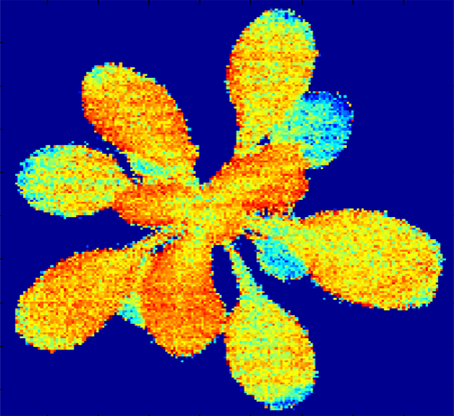
\includegraphics[width=0.35\linewidth]{example2.PNG}}\vspace{-0.1in}
\subfigure[\scriptsize Histogram of all leaves in (a)]{\includegraphics[width=0.4\linewidth]{example1-hist.PNG}}~~~
\subfigure[\scriptsize Histogram of all leaves in (b)]{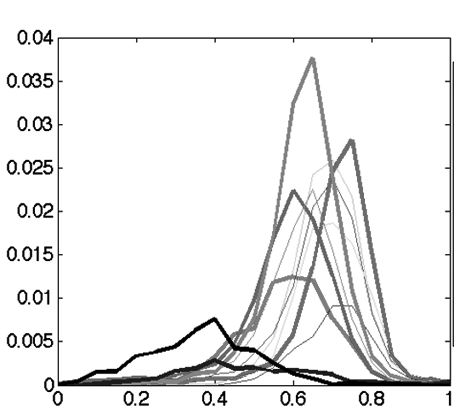
\includegraphics[width=0.4\linewidth]{example2-hist.PNG}} \vspace{-0.2in}
%\subfigure[Gene ontology (biological process)]{\includegraphics[width=0.31\textwidth]{eva_bp.eps}}
\caption{\scriptsize We demonstrate the photosynthesis heterogeneity using two Arabidopsis ecotypes (Italy and Sweden). Both plants were grown under the same stress conditions, but the false-color images of photosystem II activity shows that the Italy ecotype is more suspectable to environmental changes. \vspace{-0.3in} } \label{fig:heterogeneityexample}
\end{figure}


%Advanced technologies in high-throughput plant photosynthetic phenotyping (the Dynamic Environment Photosynthesis Imager, or DEPI) have been developed \citep{cruz2014depi,houle2010phenomics}. These systems generate huge amount of images of plant photosynthesis that can be used to quantify photosynthetic behavior in genetically diverse populations, leading to better understanding of the underlying mechanisms that control the photosynthetic properties \citep{fiorani2013future,rascher2011non}, enabling to measure variability in various photosynthetic parameters at high resolution across leaves.

%The model of spatial heterogeneity of the photosynthetic properties may reveal $CO_2$ intake capability, stomatal conductance and tolerance level to environmental changes of leaf tissues at different developmental stages.

%photosynthetic heterogeneity refers to a plant comprising multiple regions, a significant amount of which have different photosynthesis properties, %. %For example, under full sunlight photosynthesis usually captures at most only of available energy (bonner1962upper, von1981some, kramer2011importance).

Heterogeneity is a concept relating to the uniformity in a substance. The granularity of plant photosynthetic heterogeneity ranges from cells to tissues, leaves, and even the whole plant. While in-leaf variability in photosynthetic activity has been well-studied for the understanding of the effects of stomatal conductance \citep{Cheeseman1991,Buckley1997}, recent works show that photosynthetic capacity may decline with vertical gradient and leaf age \citep{Kitajima2002,chen2008effect}, suggesting that leaf-based photosynthetic heterogeneity is a key towards the understanding of plant photosynthesis.

The leaf heterogeneity in photosynthesis was firstly been studied  with a simulation model \citep{chen2008effect}. Due to the lack of high-throughput phenotyping technologies, the authors determined the effects of biochemical variability via the Farquhar model (a mechanistic, biochemical model widely used to describe steady-state $CO_2$ assimilation in leaves) incorporating defined degrees of spatial variability of its parameters~\citep{sharkey1985o2,farquhar2001models}. Spatial heterogeneity in photosynthesis was found to affect the ability of the Farquhar model to accurately characterize photosynthesis at the leaf level \citep{chen2008effect}.

Recently, with the advent of advanced technologies of biomedical imaging, directly measuring heterogeneity has recently assumed new importance~\citep{tiihonen1996cerebral,wieneke1999non,wang2000,cruz2014depi}. The rapid development of lighting and imaging techniques enables real-time non-invasive monitoring of photosynthesis \citep{houle2010phenomics,cruz2014depi}, resulting in vast amount of chlorophyll fluorescence images of plants \citep{wituszynska2013multivariable}. These images can be used to quantify photosynthetic behavior in genetically diverse populations, enabling to measure variability of photosynthetic parameters at high resolution across leaves, leading to better understanding of the underlying mechanisms that control the photosynthetic properties \citep{rascher2011non,fiorani2013future}. %However, there is no 

Measuring leaf-based photosynthetic variability in large-scale phenotyping experiments requires automatical identification of most of the visible leaves in all fluorescence images and an appropriate measurement for the variation of photosynthesis parameters across leaves that takes geometrical (leaf position and size), temporal (leaf growth rate) and physiological (leaf age) information into consideration. However, there is currently no existing infrastructure to analyze such amount of phenotype information. %The challenges of this work include not only the accurate leaf alignment in complex plant leaf layout, but also the development of a new heterogeneity measure that
%
In this paper, we present a new computational framework called {\it Plant Photosynthesis Heterogeneity} (PlantPH), and use the tool to analyze the leaf-level photosynthesis heterogeneity patterns of more than 100 Arabidopsis chloroplast mutant strains over dynamic lighting conditions, each with at least four replicates. The followed outlier detection process successfully identify mutants with distinct heterogeneity patterns under specific subsets of the environmental conditions.
%
Overall, PlantPH has the following three advantages: %The mutant screen analysis reveals that ...
\begin{enumerate}\vspace{-0.1in}
  \item~~It is the first computational framework to measure plant leaf-level heterogeneity of photosynthesis with leaf size, position and growth rate.
  \item~It's performance is significantly better than the traditional heterogeneity tests that cannot fully use the spatial and temporal information in the fluorescence images.
  \item~It discovers multiple types of photosynthetic variabilities in a large scale experiment.
\end{enumerate}

%Comparing with the existing heterogeneity approaches, our method is novel in the following ways:
%
%1.	PlantPH
%
%2. PlantPH models heterogeneity ..
%
%3. PlantPH refers to the differences between individual leaf photosynthesis and the pooled photosynthesis across all the leaves, with the weights being those used in the pooling method. With PlantPH, transient regional variation events that do not affect the whole plant photosynthesis, can be easily discovered.


%, in which hundreds of plants are screened simultaneously,
\vspace{-0.2in}
\section{Background}
The general method of assessing whether the leaves of a plant are photosynthetically homogeneous or heterogeneous is by means of the Cochran's Q-test \citep{conover1999Practical} and the $I^2$ statistic \citep{higgins2002quantifying,higgins2003measuring}. %The process has three steps.
%
%In short, the Cochran's Q-test is computed by summing the squared deviations of each object's effect estimate from overall effect estimate, weighting the contribution of each object's effect estimate by its inverse variance \citep{conover1999Practical}.
%
%The $I^2$ statistic measures the extent of true heterogeneity dividing the difference between the Cochran's Q-test value and its degree of freedom by the Q-test value \citep{higgins2003measuring,higgins2002quantifying}.
%


%and none of them can take plant specific information, such as leaf position, into the heterogeneity measurement.

%We have developed a new leaf segmentation approach called PlantPH to identify leaves from photosynthesis images...





%---------------------------
%\section{Background}
%\subsection{Heterogeneity test}

Cochran's Q-test is the classical measure of heterogeneity~\citep{conover1999Practical}. In leaf-based photosynthetic heterogeneity, $Q$ is calculated as the weighted sum of squared differences between the photosynthesis value of a individual leaf and the pooled photosynthesis value across all leaves with the weights being those used in the pooling method. The distribution of $Q$ is a chi-square statistic with $k-1$ degrees of freedom, where $k$ is the number of leaves. Cochran's Q-test has been widely used in biomedical studies. For example, heterogeneity in the aggressiveness of tumor cell populations has been adopted as an essential feature in predicting treatment success~\citep{OSullivan2003}. %However, due to the nature of plants, leaf-based photosynthetic heterogeneity often includes a small number of leaves, and thus the power of the Q-test in such circumstances could be low~\citep{higgins2003measuring, gavaghan2000evaluation}.
%
%Conversely, Q has too much power as a test of heterogeneity if the number of leaves is large \citep{higgins2003measuring}.
%
%An additional test is provided with the odds ratio meta-analysis \citep{breslow1987statistical}. It is arguably not possible to examine the null hypothesis that all studies are evaluating the same effect, by considering the only the summary data from the studies: The heterogeneity test results should be considered alongside a qualitative assessment of the combinability of studies in a systematic review.
%
The $I^2$ statistic describes the percentage of variation across studies that is due to heterogeneity rather than chance~\citep{higgins2002quantifying,higgins2003measuring}. $I^2$ can be calculated as $I^2 = (Q - df)/Q$, where Q is Cochran's Q-test heterogeneity statistic and $df$ is the degrees of freedom. A negative value  indicates no observed heterogeneity, and larger values show increasing heterogeneity. $I^2$ is an intuitive and simple expression of the inconsistency. $I^2$ of leaf-based photosynthetic heterogeneity does not inherently depend upon the number of leaves, so that $I^2$ values of different plants become comparable. A confidence interval for $I^2$ can be constructed using either the iterative non-central chi-squared distribution method \citep{hedges2001power} or the test-based method \citep{higgins2002quantifying}.

Due to the nature of plant, leaf-based photosynthetic heterogeneity often includes a small number of leaves. For example, there are less than ten rosette leaves of 2-3 week old Arabidopsis thaliana (a model plant). Thus, the power of the traditional Cochran's Q-test and $I^2$ statistic in such circumstances could be low~\citep{higgins2003measuring, gavaghan2000evaluation,huedo2006assessing,ioannidis2007uncertainty}. Furthermore, leaves may have different locations and sizes, and varying growth rates \citep{van1991insertional}, but none of them has yet been taken into the computation of heterogeneity.

Based on the rapid development in the fields of bio-imaging and computer vision, we develop a new approach called PlantPH that quantifies the effect of heterogeneity of photosynthesis across leaves of the same plant, and compare the degree of inconsistency among mutant strains in varying environmental conditions.

%To measure leaf-based photosynthetic variability in a large-scale phenotyping experiment, in which hundreds of plants are monitored in real time, it is naturally required to identify each leaf from top-view photosynthesis images automatically. However, leaf identification is a difficult task, in that 1) all the leaves are very similar in appearance especially for model plant Arabidopsis; 2) leaf features are much fewer than the well-studied face recognition problem; and 3) leaves may overlapped with each other that makes the problem more complicated. In short, there are two challenging computational problems. First, how to separate overlapped leaves in photosynthesis images where the leaf boundaries are obscure. Second, how to recognize incomplete leafs due to occlusion. Alternatively, approximation approaches can be used to estimate the leaf-based photosynthetic heterogeneity, including distribution based, region based and pixel based approaches. While these approximation approaches are easier to model, their performance may be reduced.

\begin{methods}\vspace{-0.2in}
\section{Method}\label{sec:PlantPH}




%\subsubsection*{Leaf-based heterogeneity measure}

In this article, we present a new leaf-based heterogeneity measurement, followed with a framework to efficiently use the measurement on large-scale experiments.

\subsection{PlantPH measurement}
We introduce a new leaf-based heterogeneity measurement called $PlantPH$ as follows.
%
First, let $T = \{T_{1}, T_{1}, \ldots, T_{n}\}$ be the set of effect estimates of a plant $p$ with $n$ leaves.
The effect estimate $T_{i}$ of leaf $l_i$ in plant $p$ is defined as the difference between the averaged photosynthetic values of the leaf and  the whole plant.
%
Mathematically, in each effect estimate $T_i$, let $u_i$ and $u_p$ be the averaged photosynthesis values of leaf $l_i$ and the whole plant $p$, respectively. Under the assumption of normal distribution and homoscedasticity, the effect estimate $T_i$ is the standardized mean difference \citep{hedges1998fixed}, which can be estimated by: %$T_{i} = c(l_i) (mean(l_i)-mean(p))/S(l_i,p)$ ,
%
\begin{equation}\label{eq:effectestimate}
T_{i} =  \frac{c(l_i)\left(\mu(l_i)-\mu(p)\right)}{S(l_i,p)}
\end{equation}

\noindent where $c(l_i)$ is a correction factor for the positive bias suffered by the standardized mean difference with small sample sizes, which can be estimated by $c(l_i) = 1-3/(4(|l_i|-1)-1)$ \citep{hedge1985statistical}. This adjustment will reduce the effect estimate of small leaves that only have a few pixels, and thus increase the robustness of the heterogeneity model \citep{huedo2006assessing}.
%
%According to the equation of $c(L_i, L_j)$, $c(L_i, L_j)$ is close to 1 for large leaves with many pixels, otherwise it is close to 0, down-weighing the value of heterogeneity.
%
The pooled estimate of the within-group standard deviation $S(l_i, p)$ can be computed with \citep{hedges1998fixed}:
%
\begin{equation}\label{eq:S}
S(l_i, p) = \sqrt{\frac{(|l_i|-1)std^2(l_i)+(|p|-1)std^2(p)}{|l_i|+|p|-2}}
\end{equation}

\noindent where $std^2(l_i)$ is the variance of leaf $l_i$, $std^2(p)$ is  the variance of the averaged values of all leaves in plant $p$, and $|p|$ are the total number of pixels of leaf $l_i$ and the whole plant $p$, respectively.

%The sample variance of $T_{ij}$ is estimated using Equation \ref{eq:ST} \citep{hedges1998fixed}.
%
%\begin{equation}\label{eq:ST}
%ST_{ij} = \frac{|L_i|+|L_j|}{|L_i||L_j|}+\frac{T_{ij}^2}{2(|L_i|+|L_j|)}
%\end{equation}

Then the Cochran's Q-test statistic for determining whether there is true leaf-based photosynthetic heterogeneity among the leaves is defined as:
%
\begin{equation}\label{eq:Q}
%Q=\sum_{i=1}^n \frac{\left(T_i-mean(T)\right)^2}{\tau^2}
Q=\sum_{i=1}^n w_i\left(T_i-\frac{\sum_{j=1}^n w_jT_j}{\sum_{j=1}^n w_j}\right)^2
\end{equation}

\noindent where $n$ is the total number of leaves of the plant $p$,  the right part of the equation is the weighted mean of effect estimates of all the leaves of the plant $p$, and $w_i=1/(\tau^2+\delta_i^2)$, where $\delta_i^2$ is the sampling variance of the effect estimate $T_i$, and $\tau^2$ is the between-study variance of all the effect estimates \citep{huedo2006assessing}.

To estimate $\delta_i^2$, the sampling variance of each effect estimate $T_i$, we use the photosynthetic value of every pixel in the high-resolution florescence images, in which the total number of samples of a plant is much greater than 1000. According to \citep{huedo2006assessing}, $\delta_i^2$ is close to 0. Hence, by ignoring the computation of  $\delta_i^2$ and replacing it with 0, we have:
%
\begin{equation}\label{eq:Q2}
%Q=\sum_{i=1}^n \frac{\left(T_i-mean(T)\right)^2}{\tau^2}
Q=\frac{1}{\tau^2}\sum_{i=1}^n\left(T_i-\frac{\sum_{j=1}^n T_j}{n}\right)^2
\end{equation}

Since both the between-study variance $\tau^2$ and the Q statistic represent the true heterogeneity among the distributions of the leaf-level photosynthesis, we move $\tau^2$ to the left of the equation and define a new measure called $PlantPH$:
%
\begin{equation}\label{eq:Q3}
PlantPH(f)=\sum_{i=1}^n\frac{\left(nT_if(l_i)-\sum_{j=1}^n T_jf(l_j)\right)^2}{n^3}
\end{equation}

In Equation \ref{eq:Q3}, $PlantPH(f)$ is a measure for determining whether there is true heterogeneity among all leaves of a plant. It is independent to the total number of leaves, allowing for being comparable among different plants. We take plant leaf morphology into the plant heterogeneity test by defining $f(.)$ as a function to measure the morphological properties (e.g., the area, position or growth rate) of a piece of leaf.

Specifically, in $PlantPH(area)$ we have $f(l_i)=area(l_i)$, which measures the leaf surface area \citep{boyes2001growth,tessmer2013functional}, and in $PlantPH(growth)$ we define $f(l_i)=growth\_rate(l_i)$ by adopting a three-parameter nonlinear growth model to compute both the absolute growth rate (AGR) and the relative growth rate (RGR) \citep{Richards1959,hunt1982plant,tessmer2013functional}. Moreover, in $PlantPH(position)$, we define $f(l_i)=position(l_i)$ to be 0 if $l_i$ is at the center of the plant, and 1 otherwise, in order to measure whether the leaves with a similar developmental stage have heterogeneous photosynthetic values.

 %we apply the following approach:
%\begin{enumerate}
%  \item Let $f(l_i)$ be $position(l_i)$ which returns 0 if $l_i$ is at the center of the plant, and returns 1 otherwise;
%  \item Compute $PlantPH(position)$ using Equation \ref{eq:Q3};
%  \item Since the above computation considers the plant center, we adjust $PlantPH(position)$ by
%\end{enumerate}

%%
%We estimate $\tau^2$ using the method of moments \citep{dersimonian1986meta}:
%
%\begin{equation}\label{eq:tau}
%\tau^2 = \left\{\begin{matrix}
% \frac{\widetilde{Q}-(n-1)}{\sum \widetilde{w_{i}}-\sum \widetilde{w_{i}}^2/\sum \widetilde{w_{i}}} & \widetilde{Q}>|T|+1\\
% 0 & else
%\end{matrix}\right.
%\end{equation}
%%
%\noindent where $\widetilde{Q}$ and $\widetilde{w_{i}}$ are the results of Q test of fixed effect estimate and the corresponding weight, which is computed as:	
%
%\begin{equation}\label{eq:weight}
%\widetilde{w_{i}} = \frac{1}{std^2(l_i)+c }
%\end{equation}
%
%%[Pos(L_i)\neq  Pos(L_j)] \times
%

\subsection{PlantPH workflow}

The input to the PlantPH measurement is leaf-level photosynthesis, which relies on leaf alignment and tracking~\citep{yin2014}. %By taking the biological knowledge about the shapes of any possible leaf into account, we add flexibility to the model to fit to all the general leaves. Specifically, for leaf boundary identification, we develop a leaf symmetry based curve fitting model to define the initial shape of a leaf, and develop a plant layout based approach to define leaf tips and orientation, therefore defining the leaf initial position.  Note that since leaf is assumed to be symmetric, curve fitting could converge without large amount of training.

First of all, we have developed the leaf alignment algorithm \citep{yin2014}. The work focus on ...



\end{methods}
\section{Results}

\subsection{Arabidopsis Images}

\subsubsection{Data Acquisition and Preprocessing}

In the photosynthesis phenotyping experiment, hundreds of Arabidopsis thaliana plants (wild type and genetic variations with gene knockout) were grown side-by-side under three different light conditions (constant, sinusoid, fluctuate), for in total three days.
%
Top-view fluorescence images were collected every 15 minutes in order to observe the photosynthesis activity of all of the plants simultaneously. Each fluorescence image is a grey-scale image with a resolution of 1M pixels at 12-bit intensity.

To accurately capture the photosynthesis activities of plants from fluorescence images, a image segment method is applied to remove the background, identify every piece of leaf~\citep{yin2014}, measure the intensity of pixels on leaves, and finally convert the intensity values to the measure of four kinds of photosynthesis parameters.
%
The extracted measurements of photosynthesis parameters are presented in the form of multi-dimensional time-series, one dimension for every photosynthesis parameter.
%
%Figure ?? shows that the measurements of a photosynthesis parameter $\Phi_{II}$ at one time point are quite different for the leaves of the same plant  (i.e. plant no. 3-7 and 5-5).

\subsubsection{PlantPH on Arabidopsis data}

In this experiment, wild type (col-0) and more than 100 Arabidopsis chloroplast mutant strains were grown side by side in a dynamic light condition for 3 days from 10 days old from seedling. A top-view fluorescence image was taken every 15 minutes during the day time, in order to observe the photosynthesis activity and the growth of the plants simultaneously. The overview of the experimental results is shown in Figure ???. In total, XXX fluorescence images were collected, preprocessed and fed to $PlantPH$. Note that the averaged leaf cell size of Arabidopsis is about $6000 \mu m^2$ \citep{gegas2014endopolyploidy} and our image resolution is 3600 pixels per squared inch. Therefore, each pixel in an image is sampled from about 1000 leaf cells.

The architecture of the whole process is shown in Figure \ref{fig:architecture}. First of all, we apply a leaf alignment and tracking method that we recently developed to identify most of the leaves from the top-view fluorescence images~\citep{xi2014tracking,yin2014}, and then compute the leaf-based photosynthesis value for every leaf. In addition, we add a leaf by drawing a small circle in the center of every plant to represent the young leaves that are difficult to identify.
%
All the pixels not contained in any leaf boundary are considered as an extra leaf. A leaf is ignored if its area is smaller than the plant center circle.
%
Next, we apply $PlantPH$ to compute the heterogeneity value for every plant at every snapshot, resulting in a heterogeneity matrix $H$. Finally, we recognize heterogeneity patterns in $H$ with an outlier detection method, and visually explore them with the L'Abbe plot \citep{song1999exploring}.

The results show ...

\subsubsection{Leaf alignment and tracking}

%For completeness, we introduce the leaf alignment and tracking approach...

The chlorophyll fluorescence images are false-color images, where the light intensity of every pixel is proportional to photosynthetic efficiency \citep{toet1996new} (see Figure \ref{fig:heterogeneityexample}). Differences between individual leaves with similar photosynthetic efficiency can be subtle, making the boundaries between them difficult to define and creating a significant challenge for subsequent shape analysis. The difficulty even arises when individual leaves overlap and occlude one another in these false-color images.

We have developed a framework based on the well-known Chamfer Matching algorithm \citep{yin2014}. Multi-leaf alignment aims to segment all leaves with pre-defined leaf templates and estimate the two tip points of each leaf. The tracking algorithm consists of two steps. First, a set of leaf templates are applied to the target image to generate the same amount of leaf candidates. Second, we adopt multi-objective optimization to select a subset of leaf candidates. The objective is to select a minimal number of leaf candidates with smaller Chamfer distances to cover the test image mask as much as possible.

Multi-leaf tracking is an extension of the leaf alignment algorithm. Given a serial of fluorescence images  taken over time, we first apply the alignment algorithm to the last frame, and then continuously apply template transformation to the current leaf candidates in order to fit to the previous frame. A new objective function considering the Chamfer Matching distances, target image mask, and the rotation angels of all leaves is adopted.
%
Both the leaf alignment and leaf tracking directly benefit the study of leaf behavior in plant biology, such as leaf growth, leaf-level photosynthesis, leaf-level variations in plant mutant, etc.


\subsection{PlantPH on synthetic data}

A set of synthetic data were generated to test whether $PlantPH$ is properly designed.

%\section{Materials and Methods}






% Results and Discussion can be combined.

%\subsection{Outlier detection}
%
%%Three outlier detection methods were adopted to...
%
%An outlier is an observation that appears to deviate markedly from other observations in the sample. Hampel (Hampel, 1971; Hampel, 1974) introduced the concept of the break-down point, as a measure for the robustness of an estimator against outliers.
%%
%The breakdown point is defined as the smallest percentage of outliers that can cause an estimator to take arbitrary large values. Thus, the larger breakdown point an estimator has, the more robust it is. For example, the sample mean has a breakdown point of 1/n, since a single large observation can make the sample mean and variance cross any bound.
%%
%Accordingly, Hampel suggested the median and the median absolute deviation (MAD) as robust estimates of the location and the spread. The Hampel identifier is often found to be practically very effective (Perarson, 2002; Liu et al., 2004).




\section{Discussion}

A consensus view of the data is that the photosynthesis ability of a plant is not uniform across the whole area (Charles 2008, Meng 2007).
%
The photosynthetic properties of plants can vary dramatically across cells, tissues, and organs~\citep{}, reflecting differences in development, stress responses, regulation of processes such as stomatal conductance~\citep{}, photodamage~\citep{}, and storage of photosynthate~\citep{} and contribute substantially to productivity~\citep{}.

For example, we observed that the acclimation of photosynthesis in response to cold temperatures appears to be more rapid and robust in younger or emerging than older leaves, and ecotypes isolated from different latitudes show distinct heterogeneity patterns, implying that these responses are important for adaptation of photosynthesis to fluctuating temperatures.
%
In other cases, exposure of plants to fluctuating light resulted in loss of photosynthetic capacity or increased photoinhibition in specific sets of leaves or leaf sectors. In many cases, older leaves are preferentially affected, suggesting that resources for maintenance or acclimation responses are preferentially directed to younger leaves. However, we have also identified mutant lines where younger leaves are preferentially affected, which presumably affect the development of photosynthetic robustness.

In order to systematically study the leaf level photosynthesis phenotypes, especially in a high-throughput screen manner, we developed a novel computational tool to automatically conduct statistical analysis on leaf based photosynthesis.

In the future, we will consider more plant-specific constraints including leaf shape similarity and symmetry.


\section*{Acknowledgments}\scriptsize
This research was supported by Chemical Sciences, Geosciences and Biosciences Division, Office of Basic Energy Sciences, Office of Science, U.S. Department of Energy (award number DE-FG02-91ER20021) to JC and DMK.

\bibliographystyle{natbib}

\scriptsize
%\bibliographystyle{plain}
\bibliography{heterogeneity}

\end{document}

